\documentclass[12pt]{article}
\usepackage[utf8]{inputenc}
\usepackage{biblatex}
\usepackage{graphicx}
\usepackage{amsmath}
\usepackage{amsfonts}
\usepackage{amssymb}
\usepackage{titlesec}
\usepackage[T1]{fontenc}
\addbibresource{references.bib}
\linespread{1.25}
\usepackage[lmargin=1.5in, rmargin=1.5in, tmargin=1in, bmargin=1in]{geometry}


\title{Thesis Report}
\date{April 2017}
\author{Kevin Zhu}

\newlength\tindent
\setlength{\tindent}{\parindent}
\setlength{\parindent}{0pt}
\renewcommand{\indent}{\hspace*{\tindent}}
\setlength{\parskip}{1em}

\begin{document}

\begin{titlepage}
   \centering
   {\Large\bfseries Geospatial Prediction of Donations Solicitation with Bayesian Data Fusion\par}
   \vspace{1cm}
   {by\par}
   {K. Zhu\par}
   Supervisor: Scott Sanner \par
   April 2017\par
\end{titlepage}

\newpage
\tableofcontents

\newpage
\listoffigures

\newpage 
\listoftables

\newpage
\vspace*{\fill}
{\centering\huge\bfseries Acknowledgement\par}
\bigskip
\noindent I would like to give a huge thanks to Scott Sanner for his undying support, creative drive and mentorship, making this thesis experience one to remember. He has taught me invaluable lessons in data science and machine learinng, which will be extremely useful in my future career pursuits. I would like to thank my parents for supporting me throughout University, allowing me to achieve great heights and culminate my learning into this final year thesis. 
\vspace*{\fill}

\newpage
\section{Abstract}
There are hundreds of charities that need physical donations in order to keep their cause afloat; however, there is much friction for users to donate, mostly because audience targeting is difficult. Modern platforms like Facebook allow for demographics targeting, but there is no assurance of success, leaving work mostly to expensive and resource-intensive guessing and checking. With no single data set or commercial resource to provide predictions of success, one would have to collect data from a number of different sources. Publicly available data can be highly aggregated and not conducive to traditional machine learning methods, but by means of Bayesian Data Fusion, it is possible to deaggregate this data to produce predictions that charitable organizations can rely on to effectively target their audience and boost donation numbers. 

\newpage
\section{Introduction}

% Message: You need to target a specific audience
% Current situation
With hundreds of charities and organizations seeking to help the less fortunate, donations are a key piece in keeping these groups operational and able to make significant societal contributions. While some funds like the Princess Margaret Cancer Foundation are mostly a monetary donation-based charity, others like Toys for Tots and local shelters rely heavily on physical items. Because people are not spending their resources for a return, like shopping, there is much user friction that organizations must alleviate in order for them to acquire these resources \cite{npwd}. 

% What we're doing - Making individual and location predictions possible
One of the key steps that organizations must get right is communicating their value proposition to the appropriate crowd. If they do not target the appropriate audience, soliciting donations would be nigh impossible. While it is obvious that soliciting baby goods from a region consisting mostly of University students is fruitless effort, it becomes much more difficult to make predictions of appropriate target audiences and target locations over a large number of less obvious item categories. 

% Current resources for targeting - The gap
The most modern method of soliciting goods is through online advertising platforms like Google Ads and Facebook Advertising. Physically mailing, posting on public bulletin boards, and public donation boxes have very clear drawbacks because of the amount of time their execution demands. While advertising platforms allow for wide demographical targeting based on desired audience age, gender, estimated income level, and family size, the organizations utilizing these platforms do not have any way to gain certainty that they are indeed targeting the right people. Moreover, they have no idea which parts of the city to target, forcing them to go with the blanket approach of soliciting goods from everybody. While this can easily be done on online platforms (albeit at a higher cost), physically blanketing the cities in advertisement requires a great amount of volunteer manpower that organizations may not be able to afford. 

With no single resource that charitable organizations can consult, they are hard pressed to gather data by themselves and attempt to translate into a tangible likelihood of their advertising success. 

The two basic sets of data that the charitable organizations would need are a source for item availability and a source describing the people making these items available. This would give them an idea of what items are readily accessible as well as insight as to why people make these items available in the first place. For the sake of easing data collection and analysis of the thesis, Craigslist posts were used as a measure of item availability in the city. Though the local classifieds platform is not quite representative of what people may give away to charitable organizations, the data fusion techniques can be applied all the same to a different, similarly structured, data set. Information about various target audience groups are to be retrieved from Toronto's 2014 publicly available census data (the latest available), containing aggregate statistics of individuals based on age, housing, and family size. 

% Introducing data fusion
The first thought that may come to mind is to decompose the data into features that define different members of the audience and subsequently apply an off-the-shelf machine learning technique to learn what makes different audiences unique. This type of methodology, however, requires a very granular data set where sets of features describe an individual. Companies like Facebook and major banks have access to this kind of data describing people on an individual level; however, this is rarely made available to third parties due to its sensitive nature. As a result, charitable organizations will have to rely on publicly available aggregate data sets like census data in order to gain information on various target audiences. A much less used, but arguably more valid and structured model known as a Bayesian Network can be used to fuse aggregate data sets and make much more grounded predictions on an individual level.

The thesis will explore the advantages of Bayesian data fusion and prediction on a granular, individual level over traditional machine learning models. 

\newpage
\section{Past Work} % This is the lit review
While there has not been much study conducted on the methods best for the solicitation of donations, there's much research on methods to help with geospatial predictions in ecological studies. There has also been much research into Bayesian data fusion; however, this is done mostly in the context of sensors, and not with data sets. 

A conference presentation outlines the vast capabilities of machine learning and targets it towards geospatial prediction \cite{confpres}. Because of the vast number of variables present in geospatial problems, machine learning models tend to find patterns and learn them very effectively. The presentation notes the possibility of training models using census data, allowing for fire risk to be predicted in Manhattan based on income, age and rent. The approach is heavily relevant to the thesis, as census data of Toronto can be used to predict goods availabilities throughout the city. The caveat to this paper's approach, however, is that the geospatial data used in the study was quite granular. Maps are broken down into hundreds of polygons, each having many features tied to it. 

Another paper in the field of geospatial prediction studied the link between population dynamics with climate change. They observed population features such as population growth, migration, urbanization, aging and household composition \cite{popdyn}. The paper investigates different feature sets to aid the trend of climate change. The concept of feature extraction and investigation gives rise to the idea of cross referencing patterns characterized by a particular data set (climate change in this case) with a variety of feature sets. 

Past research has utilized data fusion in three different abstraction levels \cite{df1} for decision making: low, intermediate and high. Low level data fusion is essentially the pooling of information from the sources in order to achieve a more robust, feature-rich data set for later processing and interpretation. Bayesian data fusion techniques see much use in these multisensor and data-rich environments in order to obtain a clearer, more descriptive picture of the situation\cite{sf1}.  As the levels get higher, the granularity of data decreases towards more macroscopic, decision-based data. 

Each paper was crucial to the overall understanding of the manipulation of geospatial elements with data for predictive purposes. Machine learning algorithms are simple to implement on problems with geospatial context due to the abundance of features that are present; however, it's evident that the studies had the luxury of using rich and granular data for their predictions. It would of great value to the machine learning community to explore alternative models like the relatively unexplored Bayesion data fusion technique in order to observe whether the shortcomings of aggregate data can be overcome. 

\newpage
\section{Background Information and Terminology}
There are a number of off-the-shelf machine learning models provided by libraries like python's scikit-learn and Google's TensorFlow to fit the gathered dataset. These models fall under two major categories: discriminative and generative. 

\subsection{Discriminative models}
Discriminative models take in training data and learn the features that separate different classes. Subsequent test data is then taken by the model, after which it determines the class that would most likely result. Models like Logistic Regression, Support Vector Machines, and Neural Networks are common examples. This thesis will be making use of Logistic Regression to perform the predictions. 

% Explain the Logistic Regression
\subsubsection{Logistic Regression}
Logistic regression uses the sigmoid function coupled with a linear function of multiple independent variables to ultimately determine a binary outcome. The sigmoid function is as follows: 
\[y = \frac{1}{1+e^{-z}}\]
The z is a linear function of the form
\[z = \beta_0 + \beta_1*x_1 + \beta_2*x_2 + \beta_3*x_3  + ...\]
The \(x\) values represent independent variables. The \(\beta\) values represent the weights associated with each \(x\) value. The sigmoid function can be used to calculate the probability of the outcome being 0 or 1. Training is done by feeding in a test set consisting of vectors of x values as well as the target y. Through the process of gradient descent, the model will learn the weights \(\beta\) in order to find the optimal linear boundary between the data. For testing and prediction, the model would take a vector of independent variables, apply the learned weights, the sigmoid function produces a value between 0 and 1 representing the probability of the event. A threshold, which is usually 0.5, can be applied such that beyond the threshold, the probability maps to an output of 1 and the reverse maps to an output of 0. 

\subsubsection{Multiclass Logistic Regression}
Multiclass logistic regression is an extension of logistic regression where the output can be more than just 0 and 1. It is essentially the combination of numerous logistic regression models, each of which has a set of weights allow it to predict the probability of a certain class. 

\[z = \beta_1_0 + \beta_1_1*x_1 + \beta_1_2*x_2 + \beta_1_3*x_3  + ...\]
\[    \beta_2_0 + \beta_2_1*x_1 + \beta_2_2*x_2 + \beta_2_3*x_3  + ...\]
\[    \beta_3_0 + \beta_3_1*x_1 + \beta_3_2*x_2 + \beta_3_3*x_3  + ...\]


The output becomes a vector of probabilities for each possible output class. The softmax function, or the normalized exponential function, is used to get the probabilities of each class. The maximum probability would indicate the most likely class, and therefore that class would be the output of MCLR. The softmax function looks like the following: 
\[Pr(Y_i = K) = \frac{e^{\beta_K} \cdot X_i}{\sum_{k=1}^{K} e^{\beta_K} \cdot X_i}\]

\subsection{Generative models}
Generative models train on the data and are subsequently able to provide a full probabilistic model for all the variables used in the training. As a result, in contrast to discriminative models, the generative counterpart takes in a sample test point and outputs the probability that the model would have generated the point. Classification of a point can be done with multiple generative models by obtaining the probabilities for each and assigning the point to the one with the highest probability. % Wording 
This thesis will be making use of Bayesian Networks (or Bayes net for short), as a generative model to perform predictions. 

\subsubsection{Bayesian Networks}
A Bayesian network is a graphical model that uses Bayes Rule to connect its components, or "nodes". These nodes represent pieces of information, with edges connecting different components symbolizing their relationships to one another. What results from the nodes and connections is a directed graph. 

Bayes rule is a formula that describes how likely a certain event would occur based on a certain condition, without having to know the probability of the two events occurring together. 
\[P(B_1|A)=\frac{P(B_1\cap A)}{P(A)}=\frac{P(B_1)P(A| B_1)}{\sum_{i=1}^{n} P(B_i)P(A|B_i)}\]


\begin{figure}[h]
\centering
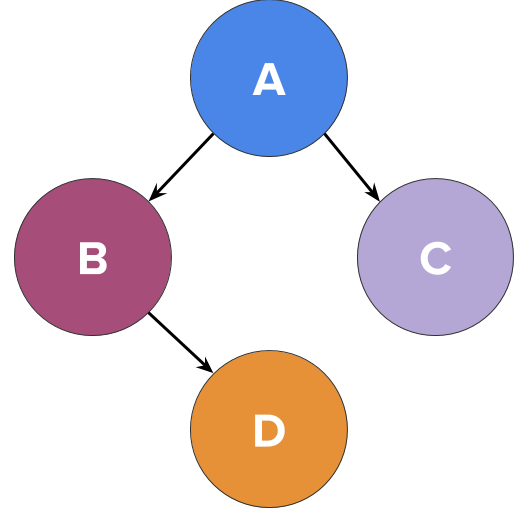
\includegraphics[width=7cm]{simple_bayes2.png}
\caption{\textit{A general bayes net. Each arrow points to the node that is conditionally dependent on the arrow source.}}
\end{figure}

In the figure, node B is conditionally dependent on node A, node C is conditionally dependent on A, and node D is conditionally dependent on B. The joint probability of the 4 events is represented by 

\[P(A,B,C,D) = P(A)P(B|A)P(C|A)P(D|B)\]

Any sort of query about the combination of variables can be made on the Bayesian Network model. For example, one could find P(D|B) through a process known as variable elimination, which essentially makes use of the law of conditional probabilities to sum out variables not found in the query to ultimately return a probability of the occurrence of event D given prior knowledge of the event B. 

\newpage
\section{Experimentation}
% How the thesis will approach data fusion
The sets of data being fused for prediction are a collection of Craigslist "item for sale" item postings in the city of Toronto and the 2014 Toronto census data. These two data sets are required to get a fundamental understanding of the charitable organization's potential target audiences. The problem that arises with solely using Craigslist is that the only useful information taht can be used is the post geotag and category. With no other pieces of information regarding the poster available, one would not be able to go beyond basic clustering and heatmapping to make predictions based on category hotspots. This result wouldn't give much insight, and organizations would just be able to post up their donation boxes in the center of the hotspot---hardly an improvement. In order to see a more complete picture of their target audience, organizations will need a demographics-related data set to fuse with the posting data set. The 2014 Toronto Census data set provides a rich, albeit aggregated, data set with the population distributions over its 44 wards of features such as age, people's housing situations, family sizes and male to female rations.

With the collected data, the popular off-the-shelf machine learning algorithm, multiclass logistic regression, will first be applied and investigated in terms of its effectiveness. Afterwards, Bayesian data fusion will be applied and subsequently compared in terms of individual prediction capabilities. 

\subsection{Data collection}
% Why Craigslist?
The data collection would be done on a single website to eliminate data format inconsistencies, productivity differences and possible overlaps in content between different websites. If additional time were taken to format and clean different posting data sets and merge them into one homogenous resource, a larger data set can be crafted. This additional work, however, is beyond the scope of the thesis. One could gather data from Ebay and Amazon; however, the postings are mostly from larger vendors, which is not suitable for individual predictions. Craigslist and Kijiji, on the other hand, are suitable because they are well known as "local classifieds", allowing anyone to post item listings for free, thereby creating a huge resource for individual item availabilities. Craigslist was chosen for data collection for its simple and easy to scrape user interface, its incredible posting throughput, and its separation of individual sellers and retailers under the guise of individuals.

% How to scrape
In the Toronto region, Craigslist gets around 2500 "item for sale" posts every two hours, each of which are bucketed into 1 of 78 categories (such a furniture, baby clothing, etc). The data collection was done via a python script, making use of a Craigslist wrapper written by Julio Malegria \cite{clwrapper} which abstracts the interface and makes automated post querying easy. 

% Troubles with the data gathering
There are a couple of caveats with using the scraper. First, there is only a total of 2500 postings at any given time that is visible on the home page. New posts bump the last post off the front page, making it invisible to the scraper. Because of the fact that it is impossible to search the entire history of Craigslist, there is the possibility that many latent variables in posting patterns would have an impact on the data gathered. In order to safely ignore the possibility that these factors exist, data was scraped from Craigslist every day at 3:00 am. The website also makes a great effort to prevent users from making a large number of requests to its website, which may cause a denial of service. As a result, they IP-ban computers that make more than a certain number of requests in a set amount of time or more than a certain number of total requests in a day. The scraping effort had to be sharded onto different machines and executed using cron jobs in order to get around this issue. A total of 55000 data points were scraped over a period of a month. 

%What does the data look like?
The most important parts of each post collected by the scraper consist of: the description of the item in the form of a title, geotags indicating the location at which the item is being sold, the url to the posting containing its designated category as well as a a timestamp indicating when it was posted. The category, a three letter code, can be extracted from the URL and aids in the bucketing of posts without the need for description processing. The geotag provides information key to helping organizations learn where to position their efforts. While the timestamp can allow for temporal analysis, the restrictions that Craigslist objection to constant data collection makes this difficult, and thus will not be explored. 

For the purpose of this thesis, it is assumed that the demographics of Toronto have not changed significantly since 2014. This assumption is not very significant in its impact on the final results, since the focus is on the fusion of this data set with the Craigslist data set. With the knowledge of posting locations, we can cross reference the geotag with a detailed, albeit aggregated census data set. The census data provides counts for different age groups, gender, household type and family size. These numbers can be normalized with respect to each ward to create ward profiles, thereby removing discrepancies between wards caused by differing populations. Consequently, a clearer demographics profile can be achieved. The age and gender feature sets are split into buckets, whereas household type and family size are split into type and size buckets respectively. 

\begin{figure}[h]
\centering
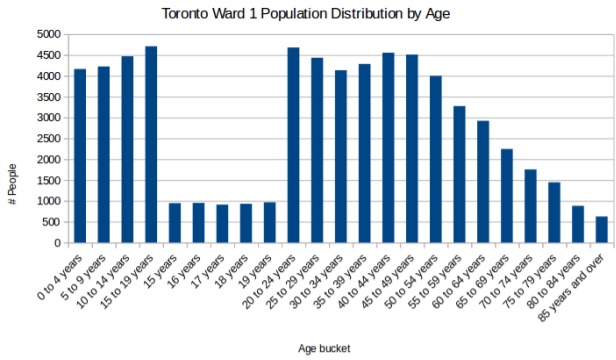
\includegraphics[width=14cm]{ward_prof1.png}
\caption{\textit{Ward 1 age distributions.}}
\end{figure}


\subsection{Initial Data Exploration}
Before any machine learning algorithm is applied, the data sets were inspected for learning potential. Great variety and granularity is a good sign that models can learn to distinguish the different classes of postings. 

Geotags associated with the post are granular enough such that the postings do not get geospatially bunched together. It would also be helpful describe places in Toronto beyond the most well known areas, so if the geotags are not specific enough, it would be nigh impossible to learn geospatial patterns. Categories, for example, serve as a good bucketing system for Craigslist postings. A very detailed timestamp is also required so that temporal analysis can be done is a possibility for future work and investigation. There is also a great distribution of data across the city of Toronto, which can be seen in figure \ref{fig:heatmap}. % TODO: WORDING

\begin{figure}[h]
\centering
\includegraphics[width=14cm]{raw_clothing.png}
% \includegraphics[width=6cm]{predicted_clothing.png}
\caption{\textit{Raw postings of the clothing category heatmapped over Toronto.}}
\label{fig:heatmap}
\end{figure}

% What was performed on the data? How was it prepped?
The first level of data processing was associating each scraped post data with one of the 44 wards in Toronto. Due to the highly irregular shaping of the Toronto Wards, association was done using nearest neighbours approach. Each posting's geotag allows for the search of the closest ward centroid. While this may not be entirely accurate, it is a very cheap and efficient way of bucketing the posts. 

\begin{figure}[h]
\centering
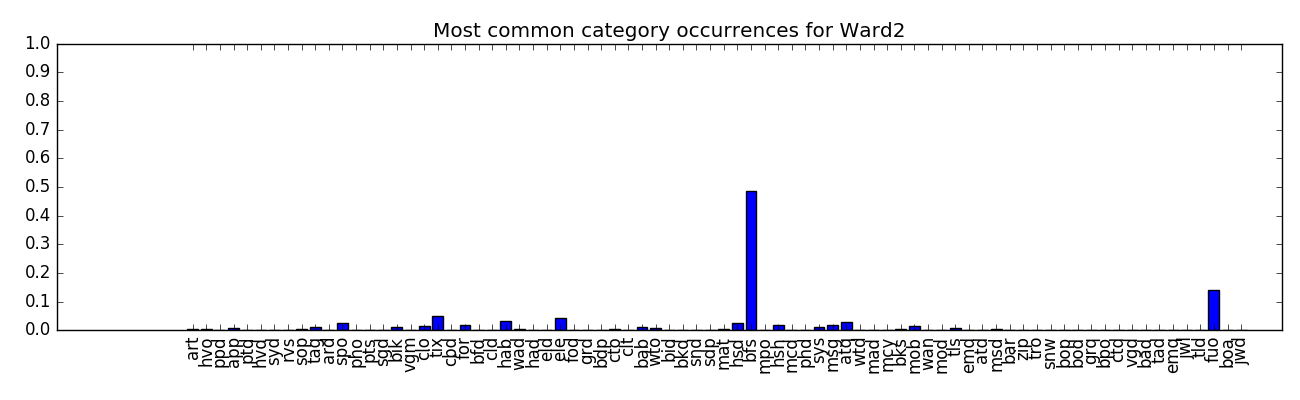
\includegraphics[width=14cm]{Ward_2.png}
\caption{\textit{Categories of postings in ward 2}}
\end{figure}

\begin{figure}[h]
\centering
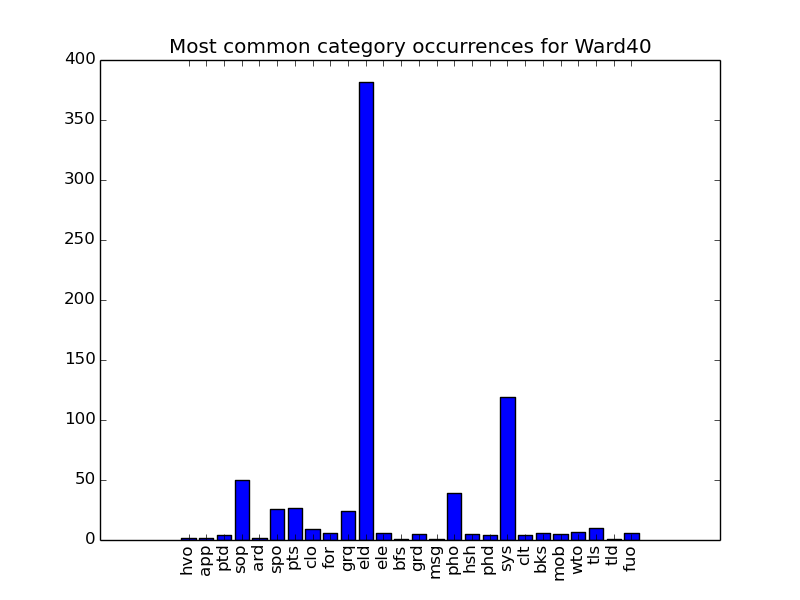
\includegraphics[width=14cm]{Ward_40.png}
\caption{\textit{Categories of postings in ward 40}}
\end{figure}

Graphing the distributions of categories of wards shows that in certain wards, very distinct peaks for different categories can be observed. This shows that there are features, latent or patent, that could help machine learning algorithms understand and predict posting locations. Had the resulting graphs shown largely random distributions of postings, it would not be immediately obvious that something could be learned by the models. 

\subsection{Multiclass Logistic Regression model training}
The first technique to model the two sets of collected data is multiclass logisitic regression. It would be trained to learn the post categories that would be most likely to spring up from a ward, providing insight into the discriminative model's ability to learn from two separate datasets.  

To train the model, a training set of 80\% of the gathered data points is used. The remaining 20\% of the data is used as a validation set. Each posts' category would be the output variable for the model: y. The independent variables or parameters, x, of the logistic regression function would collectively represent the distributions of features of a particular ward. With Toronto split into 44 wards, a feature set consisting of the normalized ward feature distributions can be constructed for each.

\begin{figure}[h]
\centering
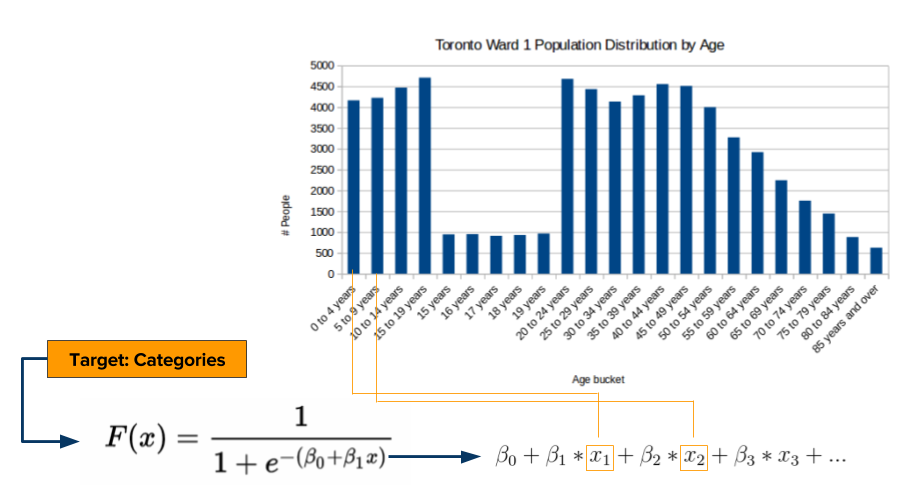
\includegraphics[width=14cm]{logistic.png}
\caption{\textit{Training of the logistic regression model.}}
\end{figure}

\subsection{Multiclass Logistic Regression Model Results}
\subsubsection{Criteria for model accuracy}
There are three methods of gauging the model accuracy in this report: raw prediction accuracy, hit rate of 5 and log likelihood. Raw prediction accuracy is measured as 
\[\text{Accuracy} = \frac{\text{Correct predictions}}{\text{Total predictions}}\]

Since the multiclass logistic regression model calculates the softmaxes for each possible class, one could count the appearance of the correct output among the top 5 of the most likely classes as a "hit". The hit rate of 5 can be calculated as follows:
\[\text{Hit Rate of 5} = \frac{\text{Occurrences of category in top five}}{\text{Total predictions}}\]

Another method of gauging model effectiveness is through negative log likelihood. This method essentially takes the negative log of the likelihood that the MCLR model gives for the correct category, and then sums it over the entire test set. With the goal of maximizing the likelihood for correct predictions, we would expect a good model to minimize the negative log likelihood and have a total of as close to 0 as possible. This method is also useful in better comparing different feature sets, as some feature sets may have poor accuracy, but they may be very confident in the predictions which turn out to be correct. This can be observed using the negative log likelihood.

\subsubsection{Multiclass Logistic Regression Prediction Results} 
\begin{figure}[h]
\centering
\includegraphics[width=14cm]{results.png}
\caption{\textit{Results of different feature sets.}}
\end{figure}
The multiclass logistic regression is able to predict the post category with almost 20\% accuracy. This is reasonable, since the model can only predict most likely categories at the granularity of a ward. 
While accuracy is important for precise predictions, it would be of great use to view the top five categories of a ward to ensure that the model is indeed learning the features that define the ward and mapping it well to the categories that the ward outputs. The hit-rate of 5 is much higher than accuracy, showing that the post category is among the top 5 most probable categories for a ward almost 50\% of the time. 

It can be observed that household type and family size overall is less indicative of categories than age and gender. The log likelihood for each feature set is a great way of checking the confidence of the models formed by different feature sets. It is possible that, despite a lower accuracy with household type and family, their correct predictions may have higher probabilities and thus a lower negative log likelihood. However, observing the negative log likelihood of the predictions by household type and family size features  reveals that this is not the case, and that they are poorer predictors with higher negative log likelihoods.

\subsection{Logistic Regression model discussion}
While the model seems to give reasonable results that are much better than the 1.28\% accuracy from purely random guessing (1/78 chance of being correct), there are two major problems with this model. The first is the inability of the model to give multiple possible category outputs per ward. Because the data describing the general population at the ward level is highly aggregated, the model can only predict one category for each ward. Without feature sets about the demographics of individuals, the model is unable to predict anything more granular than the most likely posting for the ward. This essentially makes the model worse than just picking the most common posting within a ward, which would give a 25-40\% accuracy depending on the test set. 

\begin{figure}[h]
\centering
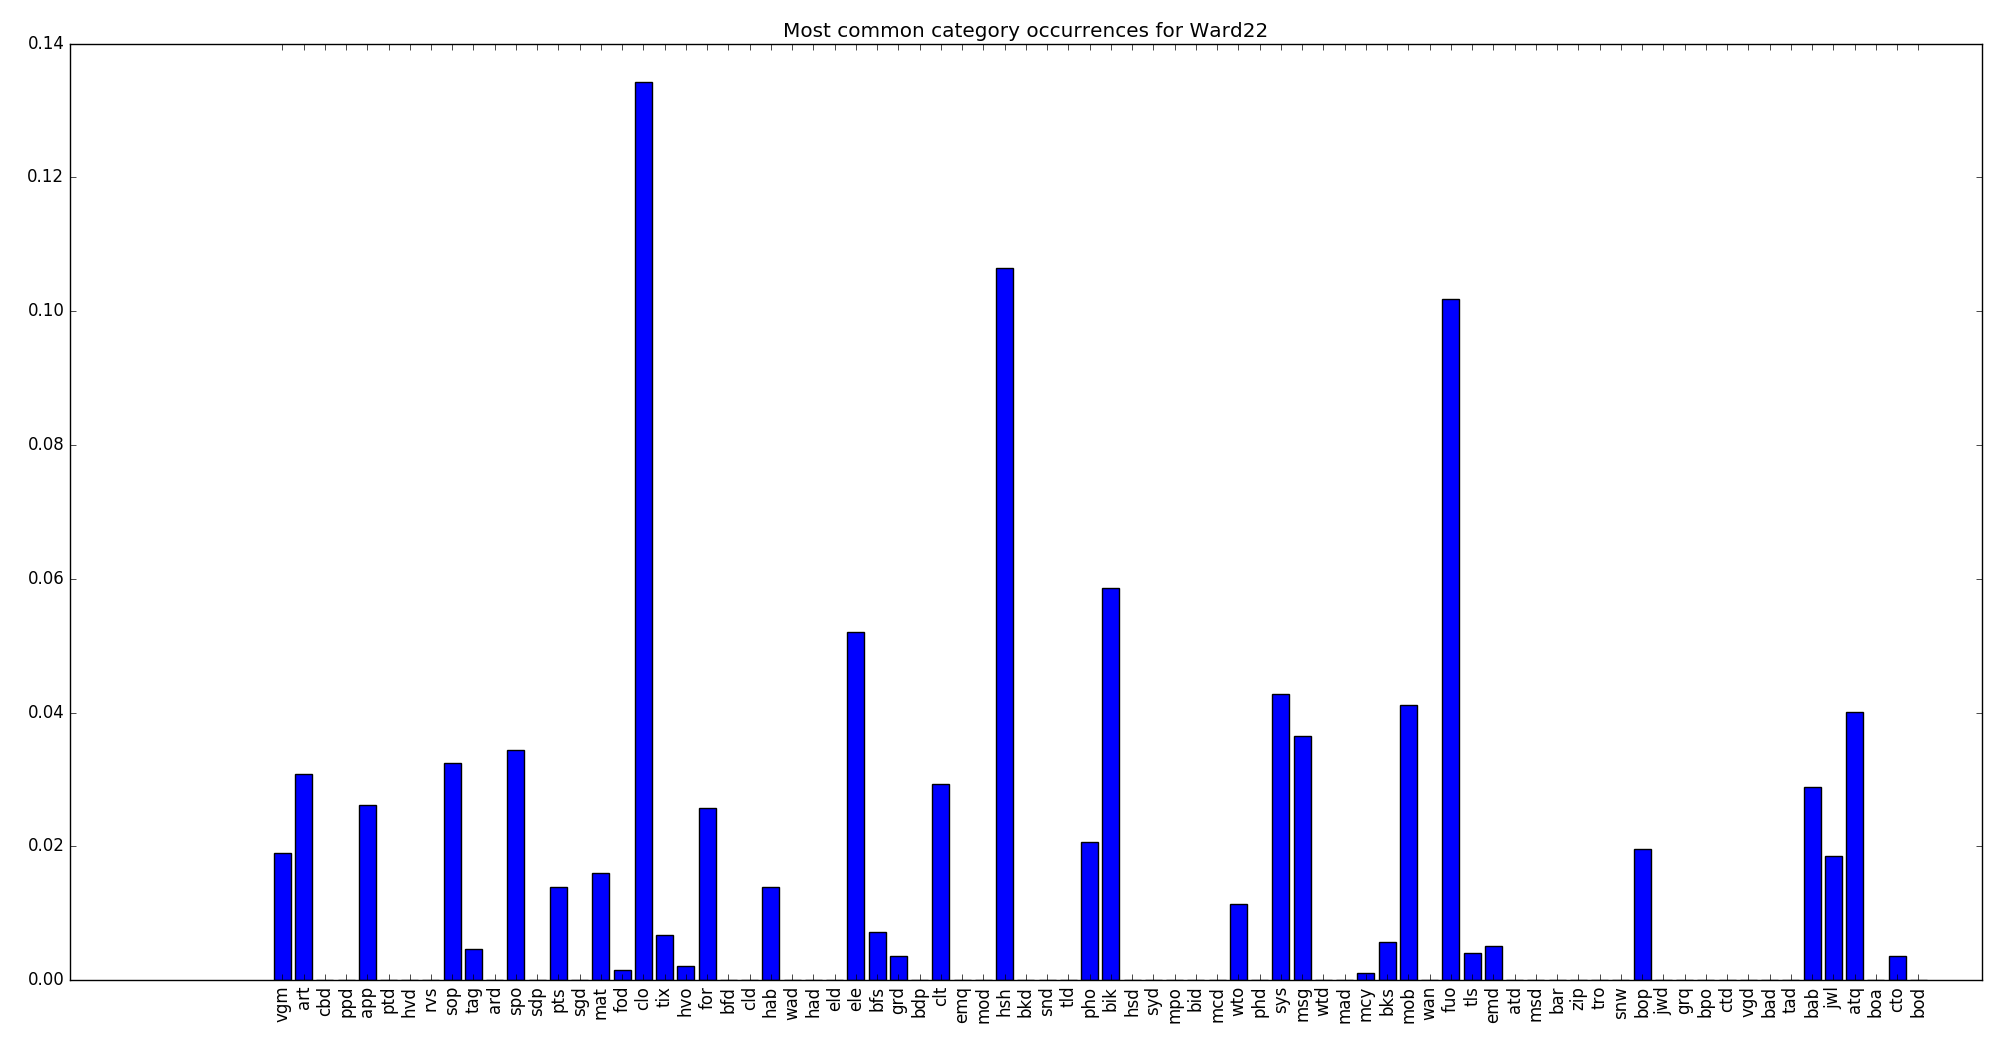
\includegraphics[width=14cm]{Ward_22.png}
\caption{\textit{Almost 50\% of the postings in ward 22 were about photo/video from dealers (phd).}}
\end{figure}

Theoretically, if the test set was composed of entirely ward 22 postings, one could predict with almost a 50\% accuracy by guessing the most common posting.

The second problem lies in the fact that, since the model is trained on aggregate data, it's only able to make reliable predictions given aggregate data as a test point. It can only reasonably know the output given the demographics of the ward. Essentially, given the resources available for training, it is impossible to make predictions given the demographics of an individual. 

While the logistic regression model is not supposed to able to predict the category for an individual, a hack can be done on the model to force a category prediction out for a particular feature bucket. This is done by a one-hot encoding of the feature input (x) for the logistic regression model. Whereas in the previous experiment in which the model would take in a feature vector consisting of the normalized values for the probabilistic distributions of a ward, this hack involves inputting a vector where a value of 1 corresponds with the desired bucket and 0 for everything else. 

\begin{figure}[h]
\centering
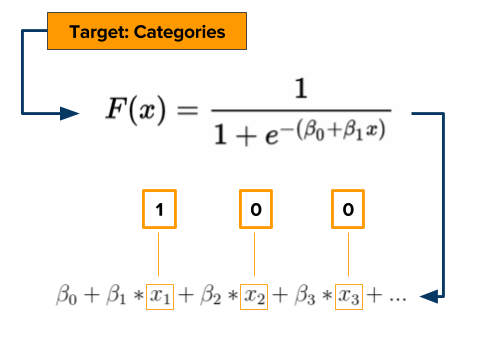
\includegraphics[width=9cm]{logistic_hack.png}
\caption{\textit{By inputting a one hot vector representing the feature bucket of interest, one could technically extract the class associated with just that feature.}}
\end{figure}

This way, the model would output a category based on knowledge about one sole feature bucket. This would allow us to compare the success of Logistic Regression and the Bayes Net on a semantically equal level. See section 5.7 for the comparison. 

\subsection{Bayesian Data Fusion --- Construction of a Bayesian model}
With just two key sources of information: postings and demographics, a simple, but powerful, Bayesian model can be constructed.

\begin{figure}[h]
\centering
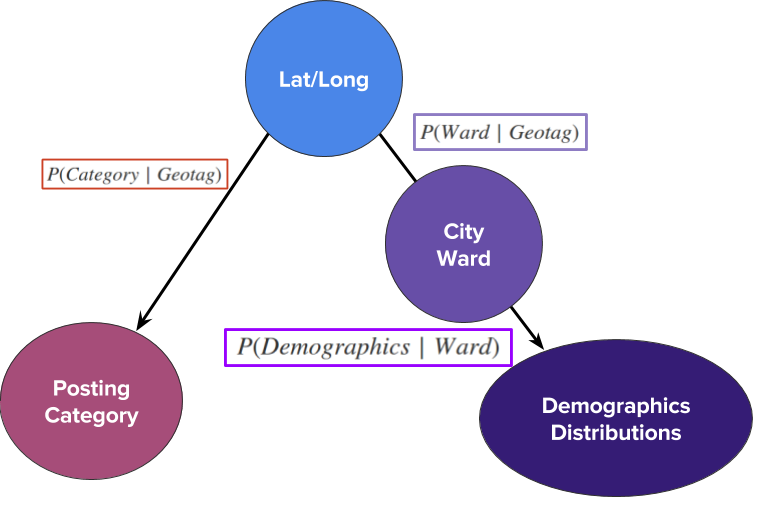
\includegraphics[width=14cm]{Bayes Net.png}
\caption{\textit{Bayesian Network showing the connections between the sets of data}}
\end{figure}

The posts and demographic distributions are connected via geotag. While geotags are much more granular, they can be brought to the ward level simply by doing a nearest neighbours approach with the centroids of the ward to find the nearest and most likely ward that the post belongs to. 
The benefit of this Bayesian model is that it basically makes individual predictions possible from aggregate data like the Toronto census, unlike the multi-class logistic regression model which can only make predictions on the aggregate data. This prediction of a category based on details of an individual essentially boils down to the following query which can be easily found with the Bayes net using the law of conditional probilities and variable elimination.  \[P(\text{category} | \text{individual demographic})\]  

\subsection{Bayesian Network and Multiclass Logistic Regression predictions on individuals}

\subsubsection{Addressing missing data needed for prediction verification}
Due to the nature of the data collected from Craigslist, there is no way to obtain the granular details of the person making a particular post. Unfortunately, without further data about the posters, it is impossible to verify predictions on the type of category posted by a particular demographic. In order to address this lack of individual details, we must simulate the data points given the currently known posting productivity within the wards as well as the demographics of the ward. 

\subsubsection{Simulation points}
The simulation points are generated using the Bayes net. From the original 55000 scraped points, we have the probabilities of certain posts originating from certain wards, as this is just basic ward productivity. First the ward origin of the simulation post is generated. From here, since category is conditionally dependent on the ward (or geotag), it is possible to generate the post category. Finally, the demographics of a person creating this post can be generated since the population probability distributions in wards is known. This process is repeated 55000 times to generate a new simulation set with information about individual demographics.

\subsubsection{Training of Bayesian and Logistic Regression Models}
Since the simulation points are generated from the Bayes Net, the conditional probibilities are known. The network only requires knowledge of these probabilities, as it was trained when the simulation points were generated. The multiclass logistic regression model was trained in the same way as with the scraped data points, using only knowledge of posting categories and the associated aggregate ward demographic. 

\subsubsection{Results and comparisons of Bayesian and Logistic Models}
Using the hack described in section 5.5, it is possible to compare the accuracy, hit rate at 5, and log likelihood of predictions between multiclass logistic regression and Bayes Net inference. The difference in results of predictions on the Bayes net versus the one-hot encoded Logistic Regression model is drastic as seen in Table 1. 

\begin{table}[]
\centering
\begin{tabular}{l|l|l|l|}
\cline{2-4}
 & Negative Log-Likelihood & Accuracy & Hit Rate of 5 \\ \hline
\multicolumn{1}{|l|}{Logistic Regression} & 47624.61 & 1.99\% & 11\% \\ \hline
\multicolumn{1}{|l|}{Bayes Net} & 24132.38 & 10.92\% & 24.6\% \\ \hline
\end{tabular}
\caption{\textit{Accuracy of category predictions on an individual.}}
% \label{my-label}
\end{table}

Here it becomes clear that due to the fact that the Logistic Regression model is trained on aggregate census data fused with Craigslist postings. The manipulation of the logistic regression model is not feasible, as it gives an abysmal accuracy that is barely better than blindly guessing the category. 

The Bayes model performs much better than its counterpart in comparison because its structure is conducive to individual queries. It still does not perform objectively well, which can be explained by the simplistic nature of the model which is composed of just 3 nodes. With more data, a more complicated model can be created, which would allow for a much more accurate prediction. 

\newpage
\section{Future Work: Considerations and experiments to perform}
In this thesis, the productivity of a ward is determined purely based on the number of people posting. This does not take negative samples into account; therefore, in our experiments, a ward making 200 posts an hour with a huge population would be considered more productive that an ward making 150 posts an hour with a much smaller population. 

A much more robust data collection tool must be developed to gather accurate and up-to-date information about the Craigslist posts. Collaboration with Craigslist to attain access to the data would be greatly beneficial, as full access to data would allow for one toachieve what was previously impossible in this thesis, such as modelling the temporal characteristics of posts. 

The current bayes net that was created is very simplistic, with just 3 nodes of importance. Since the age group distributions for each ward are not extremely distinct, it becomes very difficult to each age bucket predict a very different set of top five categories to be posted. Generating a model with data from more sources would allow it to make much more granular predictions. For example, it would be greatly useful to understand more background of the people making the post, such as occupation and features of the person's surroundings. 

\newpage
\section{Conclusion}
There is a huge advantage of Bayes model over the usual go-to off-the-shelf Machine Learning techniques such as logistic regression. When sensitive personal data can not be accessed, it becomes impossible for off the shelf machine learning algorithms like multiclass logistic regression to make granular predictions on an individual. Bayes nets, on the other hand, is able to fuse and make use of the aggregate data and deaggregate it to make predictions on a singular entity. These results have a huge impact on social service workers since they would need to have access to individual data points in order to predict their most receptive audience. Instead, they can easily make use of readily available online data to tune the targeting of their donation efforts. 

The stark contrast in predictive abilities between the discriminative methods and the generative Bayes model shows the much more principled nature of the latter model. As a result, existing data science approaches should consider the use of a more principled Bayesian approach to data fusion, as the conventional off-the-shelf classifiers and scikit-learn toolboxes may not be enough or effective for the task. 

\newpage
\printbibliography

\newpage
\section{Appendix A}
\subsection{Multiclass Logistic Regression Granularity Issues}
To visualize the predictive capabilities of multiclass logistic regression, we can heatmap the predicted postings under a particular category and compare it to the heatmap of actual postings. 

\begin{figure}[h]
\centering
\includegraphics[width=6.3cm]{raw_clothing.png}
\includegraphics[width=6cm]{predicted_clothing.png}
\caption{\textit{Left: raw postings of the clothing category. Right: predicted "hotspots" for clothing postings.}}
\end{figure}

\begin{figure}[h]
\centering
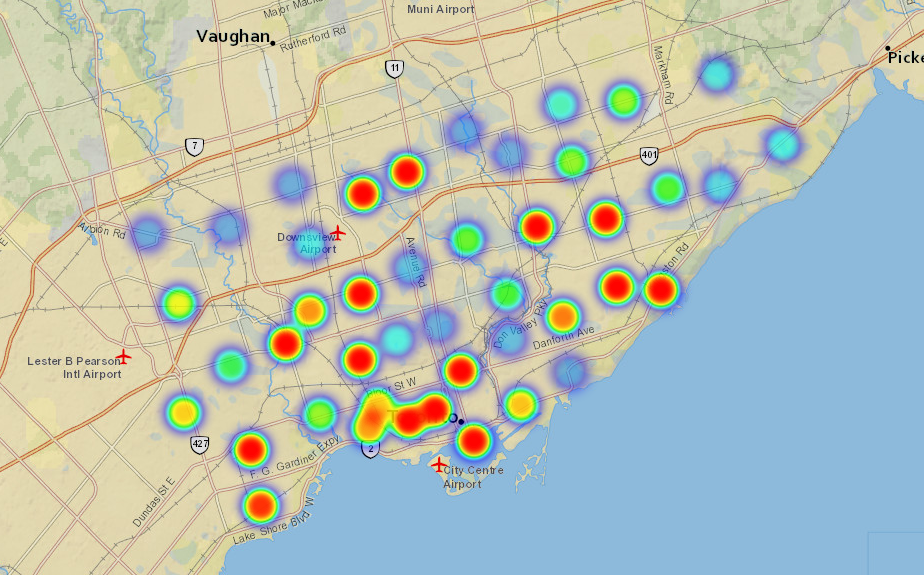
\includegraphics[width=9cm]{notgranular.png}
\caption{\textit{Zooming into the map, one can see that the predictions are not at all effective at individual predictions.}}
\end{figure}

It's obvious here that prediction by ward simply is not granular enough. As a result, it is nearly impossible to create telling heatmaps when the number of samples for a particular category is under a couple hundred. The clothings posting had over 400 posts over the course of a month, allowing for predictions to show hot spots more prominently. While it does not completely reproduce the dense hot spots in the raw heatmap, it does manage to capture and display the densest regions for clothing postings. 


\end{document}